\label{evaluation}
This chapter first compares the outcomes of the LA and the LeA. Then, the training results on different learning data sets are detailed. Lastly, the accuracy achieved by the leveraged model is compared to the accuracy attained by other projects.
\section{Clustering results}\label{clusteringEvaluation}
We compared the two used algorithms LeA and LA. The following indicators were measured. 
\begin{description}
    \item[Decomposable communities] were introduced in Subsection \ref{FEUI}.
    \item[Pages contained in decomposable communities] are pages which at the maximum zoom-level are illustrated as page-nodes.
    \item[Disconnected communities] were described in Section \ref{leidenAlgorithm}.
    \item[Total discovery time] is the time it took to detect all communities.
    \item[Highest level discovery time] is the time it took to detect the communities of the first level.
\end{description}

\begin{figure}[ht!]
  \centering
  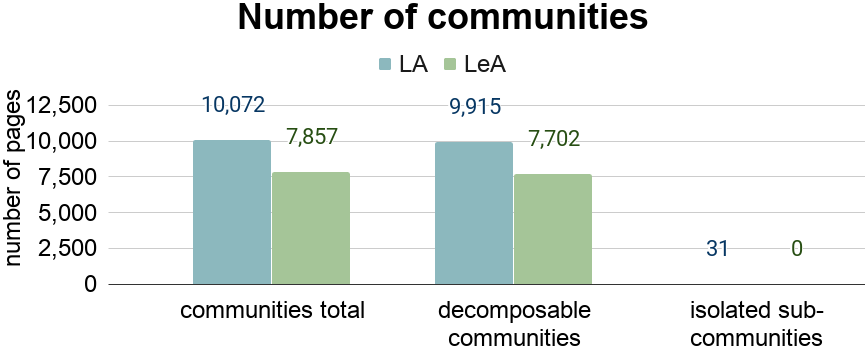
\includegraphics[width=\textwidth]{Images/CommunitiesComparison.png}
  \caption{The number of communities detected by the LA and LeA compared. }
  \label{CommunitiesComparison}
\end{figure}

\begin{figure}[ht!]
  \centering
  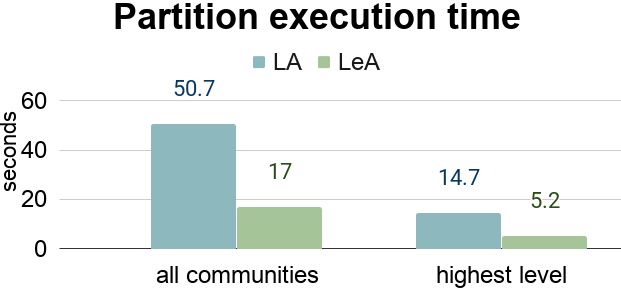
\includegraphics[width=0.8\textwidth]{Images/PartitionTimeComparison.png}
  \caption{The time it took the LA and LeA to detect communities compared.}
  \label{PartitionTimeComparison}
\end{figure}

The results are visualized in Figures \ref{CommunitiesComparison} and \ref{PartitionTimeComparison}. 

The LA detected 10,072 communities of which 9,915 were decomposable. The decomposable communities contained 33,600 pages in total. The number of disconnected sub-communities was 31. The discovering of all 10,072 communities took 59.7 seconds. The time it took to detect the communities on the highest level was about 14.7 seconds. 

The LeA detected a 7,857 communities of which 7,702 were decomposable. A total of 26,372 pages comprised the decomposable communities. No disconnected sub-communities were found. It took the LeA 17 seconds to detect all 7,857 communities. The highest level was partitioned in 5.2 seconds. 

We valued the number of decomposable communities detected by the LA. However, the disconnected sub-communities presented a problem in the correctness of the graph structure. Also, the LeA was significantly faster in detecting the communities. The algorithm used for the API responses was therefore the LeA. 

We decided to adopt LeA for the visualization of the pages on the FE. 

\section{Classification results}\label{classificationEvaluation}
Three labeled data sets were created as was described in Section \ref{LearningDatasetImplementation}. Ten independent models were trained on each data set. Another ten models were trained with pretrained embeddings on the final samples. The accuracy results of these models are depicted in this section via box plots\footnote{A visual tool for the imaged summarization and comparison of data.} \cite{boxplot}. 

The left and right sides of a box in the plot represent the first and the third quartile respectively. The vertical line inside the box portrays the median. The plus symbol in the box is the mean. The lower and upper (here left and right) whisker ends represent the minimum and maximum values respectively. The name of each box plot corresponds to the utilized training sample data set. Table \ref{categoryLegend} pairs the category shortcuts used in the plots with the actual category names. 

%\begin{wraptable}[]{l}{0.6\textwidth}
\begin{table}[H]
\centering
\scalebox{0.8}{
\begin{tabular}{@{}ll@{}}
\toprule
\rowcolor[HTML]{EEF9FB} 
{\color[HTML]{000000} \textbf{Alias}} & {\color[HTML]{000000} \textbf{Category}} \\ \midrule
\rowcolor[HTML]{DAE8E5} 
{\color[HTML]{000000} C1} & {\color[HTML]{000000} Art} \\
\rowcolor[HTML]{EEF9FB} 
{\color[HTML]{000000} C2} & {\color[HTML]{000000} Deviancy} \\
\rowcolor[HTML]{DAE8E5} 
{\color[HTML]{000000} C3} & {\color[HTML]{000000} Drugs} \\
\rowcolor[HTML]{EEF9FB} 
{\color[HTML]{000000} C4} & {\color[HTML]{000000} Encyklopedia and knowledge} \\
\rowcolor[HTML]{DAE8E5} 
{\color[HTML]{000000} C5} & {\color[HTML]{000000} Fake identity and hitmen} \\
\rowcolor[HTML]{EEF9FB} 
{\color[HTML]{000000} C6} & {\color[HTML]{000000} Finance and Fraud} \\
\rowcolor[HTML]{DAE8E5} 
{\color[HTML]{000000} C7} & {\color[HTML]{000000} Gambling} \\
\rowcolor[HTML]{EEF9FB} 
{\color[HTML]{000000} C8} & {\color[HTML]{000000} Guns} \\
\rowcolor[HTML]{DAE8E5} 
{\color[HTML]{000000} C9} & {\color[HTML]{000000} Hosting, Programming and Hacking} \\
\rowcolor[HTML]{EEF9FB} 
{\color[HTML]{000000} C10} & {\color[HTML]{000000} Online Marketplace} \\
\rowcolor[HTML]{DAE8E5} 
{\color[HTML]{000000} C11} & {\color[HTML]{000000} Other} \\
\rowcolor[HTML]{EEF9FB} 
{\color[HTML]{000000} C12} & {\color[HTML]{000000} Porn} \\
\rowcolor[HTML]{DAE8E5} 
{\color[HTML]{000000} C13} & {\color[HTML]{000000} Social} \\
\rowcolor[HTML]{EEF9FB} 
{\color[HTML]{000000} C14} & {\color[HTML]{000000} Web Catalogue} \\
\rowcolor[HTML]{DAE8E5} 
{\color[HTML]{000000} C15} & {\color[HTML]{000000} Illegal services and goods} \\
\rowcolor[HTML]{EEF9FB} 
{\color[HTML]{000000} C16} & {\color[HTML]{000000} Sexual Content} \\ \bottomrule
\end{tabular}
}
\caption{The alias-category lookup for the figures in Section \ref{classificationEvaluation}.\label{categoryLegend}}
\end{table}


\FloatBarrier

 \begin{figure}[]
    \centering
    \label{CM1Boxplot}
    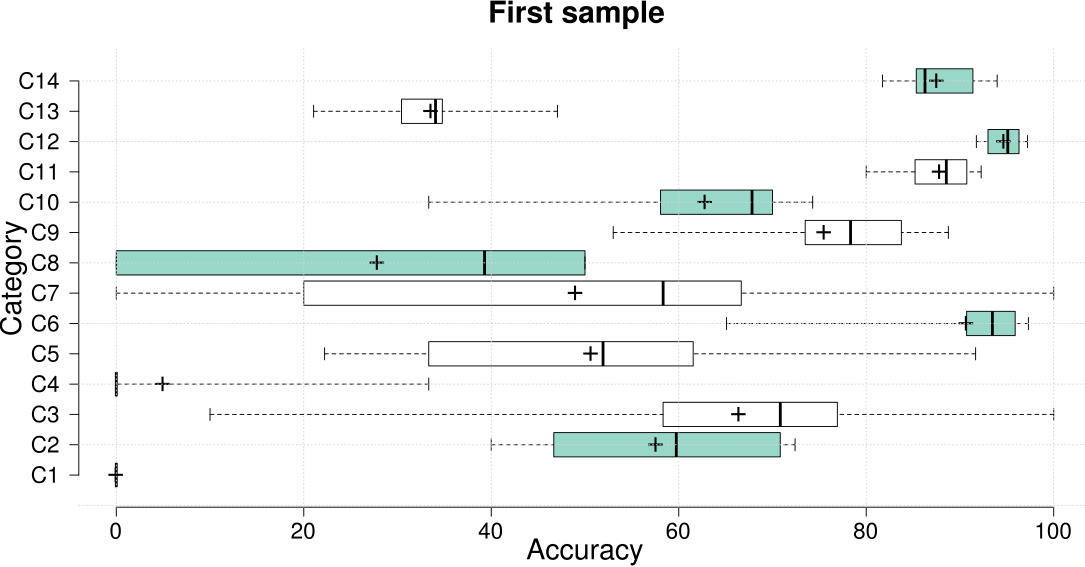
\includegraphics[width =\textwidth]{Images/CM1Boxplot.png}
    \caption{The accuracy per category of the models trained on the first samples. The median of several categories of the first samples was below 70\%. The dispersion was often over 50\%. The individual key values of this plot are detailed in Appendix \ref{CM1BoxplotValues}.}
    \label{CM1Boxplot}
\end{figure}


 \begin{figure}[]
    \centering
    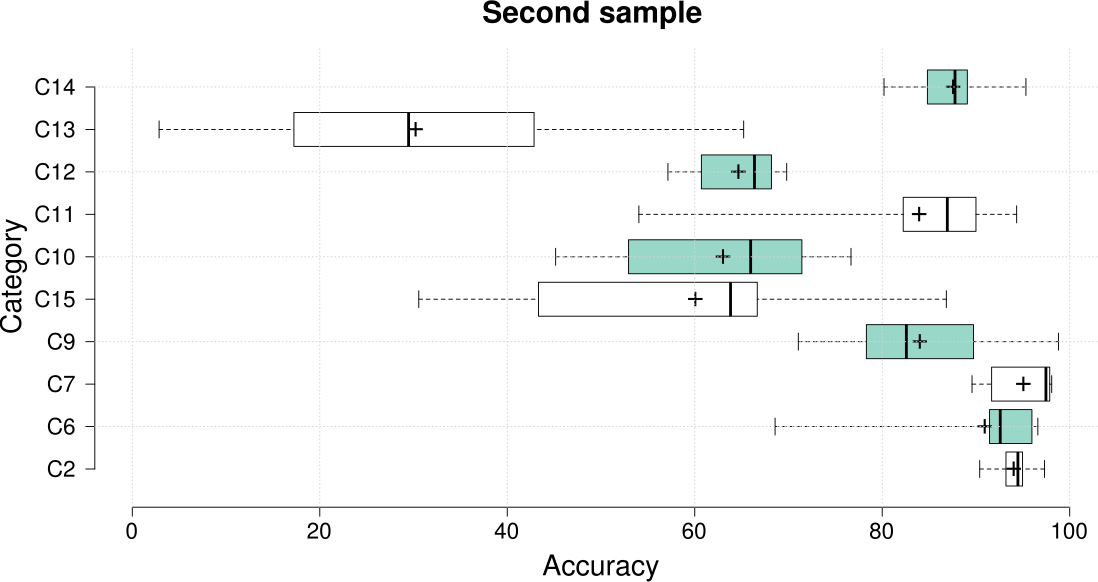
\includegraphics[width =\textwidth]{Images/CM2Boxplot.png}
    \caption{The accuracy per category of the models trained on the enhanced samples. The median of most categories was over 65\%. The dispersion was lowered. The individual key values of this plot are detailed in Appendix \ref{CM2BoxplotValues}.}
    \label{CM2Boxplot}
\end{figure}

\begin{figure}[]
 \begin{minipage}[t]{\textwidth}
    \centering
    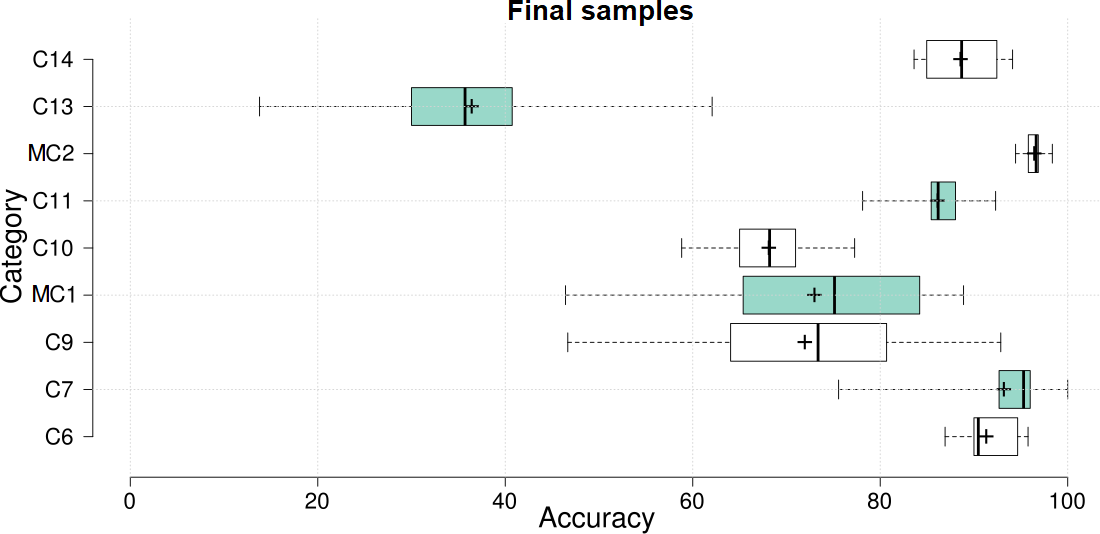
\includegraphics[width =\textwidth]{Images/CM3Boxplot.png}
    \caption{The accuracy per category of the models trained on the final samples. The dispersion was low compared to the results in the enhanced samples. The individual key values of this plot are detailed in Appendix \ref{CM3BoxplotValues}.}
    \label{CM3Boxplot}
\end{minipage}

 \begin{minipage}[b]{\textwidth}
    \centering
    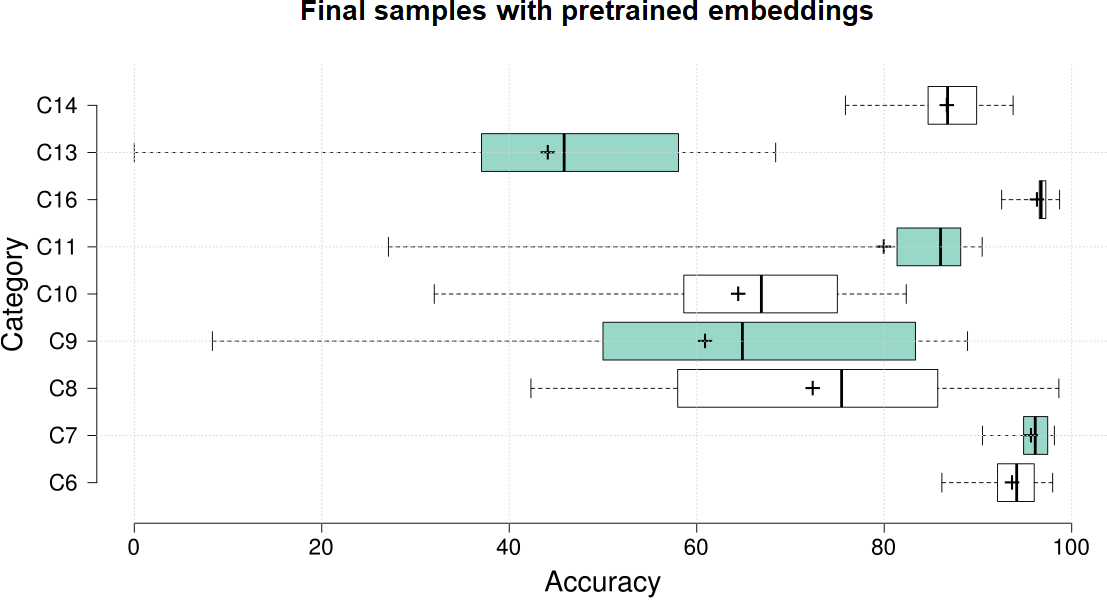
\includegraphics[width =0.95\textwidth]{Images/CM3EmbeddingsBoxplot.png}
    \caption{The accuracy per category of the models trained on the final samples with pretrained embeddings. The maximums and the third quartiles were better compared to the final samples without pretrained embeddings. However, the dispersion of the results was comparatively as bad as in the results with the first samples. The possible reasons were discussed in Subsection \ref{ClassificationImplementation}. The individual key values of this plot are detailed in Appendix \ref{CM3EmbeddingsBoxplotValues}.}
    \label{CM3EmbeddingsBoxplot}
\end{minipage}
\end{figure} \hfill

 \begin{figure}[t]
    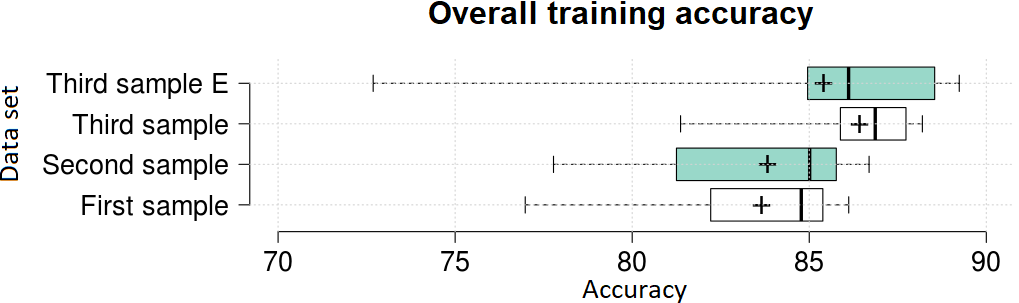
\includegraphics[width =\textwidth]{Images/DSsBoxplot.png}
    \caption{The overall accuracy of the models trained on the dataset samples described in Section \ref{LearningDatasetImplementation}. The data set \textit{Final samples E} stands for the training on the final samples with pretrained embeddings. The individual key values of box plots are detailed in Appendix \ref{DSsBoxplotValues} }
    \label{DSsBoxplot}
\end{figure}

\FloatBarrier
The learning data set used for the model training was the final samples. The final model utilized in the BE for the categorization of the pages achieved 88.2\% accuracy. We compared these results to two other projects both from the year 2017. The ATOL \cite{atol} classification tool scored an accuracy of 96.4\%. ATOL was used for the categorization of the dark web into 3 categories - drugs, hacker, weapons. The learning data set contained 529 sites. 

The second classifying tool \cite{classificationProject} we compared our results to accomplished an accuracy of 96.6\%. This tool classified the data into 9 categories. The learing approach chosen was SLr. The learning data set contained 6831 pages. 

Both other projects have achieved a higher accuracy. However, ATOL recognized only 3 divergent categories which may explain the high accuracy. The second project adopted a more sophisticated CNN and model balancing. 

